\documentclass[11pt,a4paper]{article}

% --- Page Margins ---
\usepackage[a4paper, top=2.4cm, bottom=2.4cm, left=2.2cm, right=2.2cm]{geometry}

% --- Font Configuration: Times New Roman ---
\usepackage{iftex}
\ifPDFTeX
    \usepackage[T1]{fontenc}
    \usepackage{mathptmx}
\else
    \usepackage{fontspec}
    \IfFontExistsTF{Times New Roman}{
        \setmainfont{Times New Roman}
    }{
        \setmainfont{TeX Gyre Termes}
    }
\fi

% --- Line Spacing: 20 pt (11pt default baselineskip is 13.6pt; 13.6 * 1.47 = 20pt) ---
\linespread{1.47}

% --- Math, Typography, and Layout Packages ---
\usepackage{amsmath,amssymb,amsthm}
\usepackage{parskip}
\usepackage{enumitem}
\usepackage{xcolor}
\usepackage{float}
\usepackage{tikz}
\usetikzlibrary{decorations.markings, intersections}

% --- List Spacing Refinement ---
\setlist[itemize]{itemsep=2pt, topsep=3pt, parsep=2pt, leftmargin=1.6em}
\setlist[enumerate]{itemsep=2pt, topsep=3pt, parsep=2pt, leftmargin=1.8em}

% --- Custom Theorem & Definition Styles (Header on its own line) ---
\newtheoremstyle{definitionbreak}
  {10pt}        % Space above
  {10pt}        % Space below
  {\normalfont} % Body font
  {0pt}         % Indent amount
  {\bfseries\color{blue!60!black}} % Theorem head font
  {.}           % Punctuation after theorem head
  {\newline}    % Space after theorem head (starts body on a new line)
  {\thmname{#1}\thmnumber{ #2}\thmnote{ \textnormal{\textbf{(#3)}}}}

\newtheoremstyle{examplebreak}
  {10pt}        % Space above
  {10pt}        % Space below
  {\normalfont} % Body font
  {0pt}         % Indent amount
  {\bfseries\color{teal!65!black}} % Theorem head font
  {.}           % Punctuation after theorem head
  {\newline}    % Space after theorem head (starts body on a new line)
  {\thmname{#1}\thmnumber{ #2}\thmnote{ \textnormal{\textbf{(#3)}}}}

\theoremstyle{definitionbreak}
\newtheorem{definition}{Definition}

\theoremstyle{examplebreak}
\newtheorem{example}{Example}

\theoremstyle{plain}
\newtheorem{theorem}{Theorem}
\newtheorem{proposition}{Proposition}
\newtheorem{lemma}{Lemma}

% --- Hyperref (Must be loaded last) ---
\usepackage[colorlinks=true, linkcolor=blue!60!black, urlcolor=blue!60!black]{hyperref}

\begin{document}

% ==================================================
% Title and Instructor Information
% ==================================================
\begin{center}
    {\LARGE \textbf{Mathematics Method for Physics -- Lecture 3}} \\[0.4em]
    {\large Planar Point Sets, Extended Complex Plane, and Complex Functions}
\end{center}

\vspace{-0.4em}
\noindent\rule{\textwidth}{0.6pt}
\vspace{0.1em}

\begin{center}
    Instructor: Zhaolong Han, SOCE, Shanghai Jiao Tong University \quad|\quad Email: \texttt{han.arkey@sjtu.edu.cn}
\end{center}

\vspace{0.1em}
\noindent\rule{\textwidth}{0.6pt}

\vspace{0.5em}
\noindent \textit{Overview: These lecture notes cover the topological foundations of planar point sets and domains, the extended complex plane and Riemann sphere, functions of a complex variable as geometric mappings, and the five classes of elementary complex functions.}

\vspace{0.8em}

% ==================================================
% Section 1: Planar Point Sets and Domains
% ==================================================
\section{Planar Point Sets and Domains}

\subsection{Neighborhood and Classification of Points}

\begin{definition}[Neighborhood]
The point set determined by the inequality $|z - z_0| < \varepsilon$ ($\varepsilon > 0$) is called the $\varepsilon$-neighborhood of $z_0$, denoted as $N(z_0, \varepsilon)$. Geometrically, it represents an open disk centered at $z_0$ with radius $\varepsilon$ (excluding its boundary circle). The deleted neighborhood is defined by $0 < |z - z_0| < \varepsilon$ and denoted by $\mathring{N}(z_0, \varepsilon)$.
\end{definition}

\begin{definition}[Classification of Points]
Let $E$ be a point set in the complex plane $\mathbb{C}$ and $z_0 \in \mathbb{C}$ be a point:
\begin{itemize}
    \item \textbf{Interior Point}: If $z_0 \in E$ and there exists a neighborhood $U = N(z_0, \varepsilon)$ such that $U \subset E$, then $z_0$ is called an interior point of $E$.
    \item \textbf{Exterior Point}: If there exists a neighborhood $U = N(z_0, \varepsilon)$ that has an empty intersection with $E$ ($U \cap E = \emptyset$), then $z_0$ is called an exterior point of $E$.
    \item \textbf{Boundary Point}: If every neighborhood $U = N(z_0, \varepsilon)$ of $z_0$ contains both points belonging to $E$ and points not belonging to $E$, then $z_0$ is called a boundary point of $E$. A boundary point may either belong to $E$ or not belong to $E$.
\end{itemize}
The set of all boundary points of $E$ is called the \textbf{boundary} of $E$, denoted by $\partial E$ or $\Gamma(E)$.
\end{definition}

\begin{figure}[H]
\centering
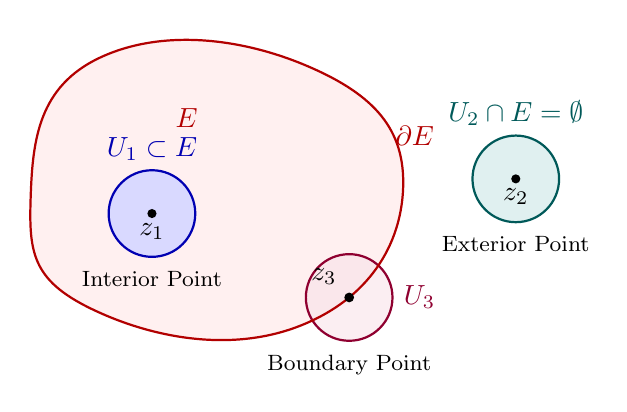
\begin{tikzpicture}[scale=1.1]
    % Domain E fill and named boundary path
    \path[name path=boundary, fill=red!6!white] 
        plot[smooth cycle, tension=0.8] coordinates {(-2,0) (-1.2,1.6) (1.2,1.5) (2.3,0.1) (1.1,-1.5) (-1.3,-1.3)};
    \node[red!70!black, font=\bfseries] at (-0.2, 0.9) {$E$};
    \node[red!70!black, right] at (2.1, 0.7) {$\partial E$};

    % Compute exact intersection point z3 on boundary of E
    \path[name path=ray] (0.5, -0.2) -- (2.2, -1.6);
    \path[name intersections={of=boundary and ray, by=z3}];

    % 1. Interior point z1
    \coordinate (z1) at (-0.6, -0.2);
    \draw[thick, blue!70!black, fill=blue!15!white] (z1) circle (0.5cm);
    \fill[black] (z1) circle (1.5pt) node[below] {$z_1$};
    \node[blue!70!black, above] at (-0.6, 0.3) {$U_1 \subset E$};
    \node[below, font=\footnotesize] at (-0.6, -0.75) {Interior Point};

    % 2. Exterior point z2
    \coordinate (z2) at (3.6, 0.2);
    \draw[thick, teal!70!black, fill=teal!12!white] (z2) circle (0.5cm);
    \fill[black] (z2) circle (1.5pt) node[below] {$z_2$};
    \node[teal!70!black, above] at (3.6, 0.7) {$U_2 \cap E = \emptyset$};
    \node[below, font=\footnotesize] at (3.6, -0.35) {Exterior Point};

    % 3. Boundary point z3 (centered directly on boundary of E)
    \draw[thick, purple!75!black, fill=purple!12!white, fill opacity=0.55] (z3) circle (0.5cm);
    \draw[thick, red!70!black] 
        plot[smooth cycle, tension=0.8] coordinates {(-2,0) (-1.2,1.6) (1.2,1.5) (2.3,0.1) (1.1,-1.5) (-1.3,-1.3)};
    \fill[black] (z3) circle (1.6pt) node[above left=1pt] {$z_3$};
    \node[purple!75!black, right] at ([xshift=0.52cm]z3) {$U_3$};
    \node[below, font=\footnotesize] at ([yshift=-0.55cm]z3) {Boundary Point};
\end{tikzpicture}
\caption{Classification of interior ($z_1$), exterior ($z_2$), and boundary ($z_3$) points with respect to set $E$.}
\end{figure}

\subsection{Open Sets, Closed Sets, and Domains}

\begin{definition}[Open Set, Closed Set, and Closure]
For a point set $E \subset \mathbb{C}$, we define the following basic topological notions:
\begin{itemize}
    \item \textbf{Open Set}: A point set $E$ is called an open set if every point of $E$ is an interior point (i.e., $E = \{ \text{interior points of } E \}$).
    \item \textbf{Closed Set}: A point set $E$ is called a closed set if its complement $\mathbb{C} \setminus E$ is an open set; equivalently, $E$ contains all of its boundary points ($\partial E \subset E$).
    \item \textbf{Closure}: The union of a set $E$ and its boundary $\partial E$ is called the closure of $E$, denoted by $\overline{E} = E \cup \partial E$.
    \item \textbf{Bounded Set}: A set $E$ is bounded if there exists a positive constant $R > 0$ such that $E \subset \{z \mid |z| < R\}$; otherwise, it is unbounded.
\end{itemize}
\end{definition}

\begin{definition}[Connected Set and Domain]
Let $E$ and $D$ be point sets in the complex plane $\mathbb{C}$:
\begin{itemize}
    \item \textbf{Connected Set}: A point set $E$ is called connected if any two points $A, B \in E$ can be joined by a polygonal line lying entirely within $E$.
    \item \textbf{Domain (Region)}: A non-empty, open, and connected point set $D$ is called a domain.
    \item \textbf{Closed Domain}: A domain $D$ together with its boundary $\partial D$ is called a closed domain, denoted by $\overline{D} = D \cup \partial D$.
\end{itemize}
\end{definition}

\begin{figure}[H]
\centering
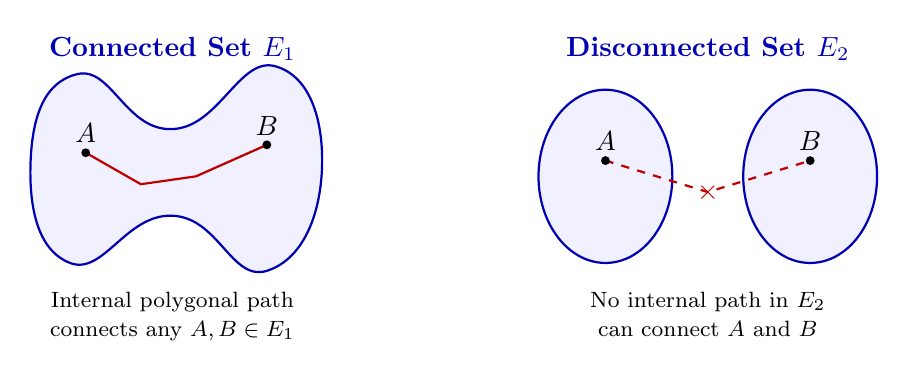
\begin{tikzpicture}[scale=1.0]
    % Left: Connected Set E1
    \begin{scope}[shift={(-3.4, 0)}]
        \draw[thick, blue!70!black, fill=blue!6!white] 
            plot[smooth cycle, tension=0.85] coordinates {(-1.8,0.2) (-1.2,1.3) (0,0.6) (1.3,1.4) (1.9,0.1) (1.2,-1.2) (0,-0.5) (-1.3,-1.1)};
        \node[blue!70!black, above] at (0, 1.35) {\textbf{Connected Set $E_1$}};
        
        \coordinate (A) at (-1.1, 0.3);
        \coordinate (B) at (1.2, 0.4);
        \draw[thick, red!75!black] (A) -- (-0.4, -0.1) -- (0.3, 0.0) -- (B);
        \fill[black] (A) circle (1.6pt) node[above] {$A$};
        \fill[black] (B) circle (1.6pt) node[above] {$B$};
        \node[below, font=\footnotesize\linespread{1.1}\selectfont, align=center] at (0, -1.35) {Internal polygonal path \\ connects any $A, B \in E_1$};
    \end{scope}

    % Right: Disconnected Set E2
    \begin{scope}[shift={(3.4, 0)}]
        \draw[thick, blue!70!black, fill=blue!6!white] (-1.3, 0) ellipse (0.85cm and 1.1cm);
        \draw[thick, blue!70!black, fill=blue!6!white] (1.3, 0) ellipse (0.85cm and 1.1cm);
        \node[blue!70!black, above] at (0, 1.35) {\textbf{Disconnected Set $E_2$}};

        \coordinate (C) at (-1.3, 0.2);
        \coordinate (D) at (1.3, 0.2);
        \draw[thick, dashed, red!75!black] (C) -- (0, -0.2) -- (D);
        \node[red!75!black, font=\bfseries] at (0, -0.2) {$\times$};
        \fill[black] (C) circle (1.6pt) node[above] {$A$};
        \fill[black] (D) circle (1.6pt) node[above] {$B$};
        \node[below, font=\footnotesize\linespread{1.1}\selectfont, align=center] at (0, -1.35) {No internal path in $E_2$ \\ can connect $A$ and $B$};
    \end{scope}
\end{tikzpicture}
\caption{Geometric comparison of connected and disconnected planar sets.}
\end{figure}

\begin{definition}[Simply Connected and Multiply Connected Domains]
Let $D$ be a domain. If for every simple closed curve $C$ lying inside $D$, the entire interior of $C$ also belongs to $D$ (i.e., $\operatorname{Int}(C) \subset D$), then $D$ is called a \textbf{simply connected domain}. A domain that is not simply connected is called a \textbf{multiply connected domain} (which contains ``holes'').
\end{definition}

\subsection{Positive Orientation of the Boundary}

For a domain $D$ bounded by one or more simple closed curves, the \textbf{positive orientation} (positive direction) of the boundary $\Gamma$ is defined such that when traversing $\Gamma$ in the positive direction, the domain $D$ always lies to the \textbf{left-hand side}.

Accordingly, for a multiply connected domain bounded by an outer simple closed curve $C_0$ and inner disjoint simple closed curves $C_1, C_2, \dots, C_n$:
\begin{itemize}
    \item The outer boundary $C_0$ is oriented counterclockwise.
    \item Each inner boundary $C_k$ ($k = 1, 2, \dots, n$) is oriented clockwise (denoted $C_k^-$).
    \item The total positively oriented composite boundary is written symbolically as
    \[
        \Gamma = C_0 + C_1^- + C_2^- + \dots + C_n^-.
    \]
\end{itemize}

\begin{figure}[H]
\centering
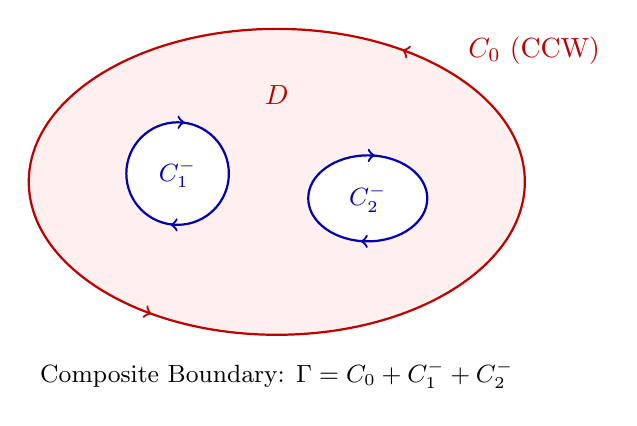
\begin{tikzpicture}[scale=1.05,
    ccw arrow/.style={postaction={decorate}, decoration={markings, mark=at position 0.15 with {\arrow{>}}, mark=at position 0.65 with {\arrow{>}}}},
    cw arrow/.style={postaction={decorate}, decoration={markings, mark=at position 0.25 with {\arrow{<}}, mark=at position 0.75 with {\arrow{<}}}}
]
    % Outer boundary C0 (CCW)
    \draw[thick, red!75!black, fill=red!6!white, ccw arrow] (0,0) ellipse (3.0cm and 1.85cm);
    \node[red!75!black, above right] at (2.2, 1.3) {$C_0$ (CCW)};

    % Inner hole C1 (CW)
    \draw[thick, blue!70!black, fill=white, cw arrow] (-1.2, 0.1) circle (0.62cm);
    \node[blue!70!black, font=\small] at (-1.2, 0.1) {$C_1^-$};

    % Inner hole C2 (CW)
    \draw[thick, blue!70!black, fill=white, cw arrow] (1.1, -0.2) ellipse (0.72cm and 0.52cm);
    \node[blue!70!black, font=\small] at (1.1, -0.2) {$C_2^-$};

    \node[red!75!black, font=\bfseries] at (0, 1.05) {$D$};
    \node[below, font=\small] at (0, -2.05) {Composite Boundary: $\Gamma = C_0 + C_1^- + C_2^-$};
\end{tikzpicture}
\caption{Positive boundary orientation of a multiply connected domain $D$ (domain remains on the left).}
\end{figure}

\subsection{Typical Examples of Planar Domains}

\begin{example}[Textbook Example 1.12]
Determine the point set $D$ defined in polar coordinates by $\cos\theta < r < 2\cos\theta$ ($-\frac{\pi}{2} < \theta < \frac{\pi}{2}$). Since $r = \sqrt{x^2+y^2}$ and $\cos\theta = \frac{x}{\sqrt{x^2+y^2}}$, multiplying by $r > 0$ yields $x < x^2 + y^2 < 2x$, which can be rewritten as
\[
    \begin{cases}
        (x - 1)^2 + y^2 < 1, \\[4pt]
        \left(x - \dfrac{1}{2}\right)^2 + y^2 > \dfrac{1}{4}.
    \end{cases}
\]
The boundary consists of two circles $\Gamma_1: r = \cos\theta$ and $\Gamma_2: r = 2\cos\theta$ internally tangent at the origin $z = 0$. The crescent-shaped open region $D$ between them is a \textbf{bounded, simply connected domain}.
\end{example}

\begin{example}[Textbook Example 1.13]
Determine the point set $D$ defined by $0 < \arg\frac{z - i}{z + i} < \frac{\pi}{4}$. Setting $z = x + iy$, we compute
\[
    \frac{z - i}{z + i} = \frac{x^2 + y^2 - 1}{x^2 + (y+1)^2} - i \frac{2x}{x^2 + (y+1)^2}.
\]
The condition $0 < \arg\frac{z - i}{z + i} < \frac{\pi}{4}$ corresponds to $0 < \frac{-2x}{x^2 + y^2 - 1} < 1$ with $x < 0$, which simplifies to
\[
    \begin{cases}
        x < 0, \\[4pt]
        (x + 1)^2 + y^2 > 2.
    \end{cases}
\]
Its boundaries are $\Gamma_1$ (the rays on the imaginary axis $x = 0$ with $|y| > 1$) and $\Gamma_2$ (the left circular arc $(x+1)^2 + y^2 = 2, x < 0$). Thus, $D$ is an \textbf{unbounded, simply connected domain}.
\end{example}

% ==================================================
% Section 2: Extended Complex Plane and Point at Infinity
% ==================================================
\section{Extended Complex Plane and the Point at Infinity}

\subsection{The Point at Infinity and Arithmetic Conventions}

To unify the behavior of unbounded sequences and mappings, we adjoin a single ideal element called the \textbf{point at infinity}, denoted by $\infty$, to the finite complex plane $\mathbb{C}$.

\begin{definition}[Extended Complex Plane]
The set $\mathbb{C}_\infty = \mathbb{C} \cup \{\infty\}$ is called the \textbf{extended complex plane}. For the symbol $\infty$, its modulus is defined as
\[
    |\infty| = +\infty,
\]
whereas its real part ($\operatorname{Re}\infty$), imaginary part ($\operatorname{Im}\infty$), and argument ($\operatorname{Arg}\infty$) are undefined.
\end{definition}

For any finite complex number $a \in \mathbb{C}$, arithmetic operations involving $\infty$ are governed by the following rules:
\begin{enumerate}
    \item $a \pm \infty = \infty \pm a = \infty$;
    \item $a \cdot \infty = \infty \cdot a = \infty$ \quad ($a \neq 0$);
    \item $\dfrac{a}{\infty} = 0$, \quad $\dfrac{a}{0} = \infty$ \quad ($a \neq 0$).
\end{enumerate}
The expressions $\infty \pm \infty$, $0 \cdot \infty$, $\dfrac{\infty}{\infty}$, and $\dfrac{0}{0}$ remain indeterminate and meaningless. Note that unlike the extended real line $\mathbb{R} \cup \{-\infty, +\infty\}$, the extended complex plane $\mathbb{C}_\infty$ contains \textbf{only one} point at infinity.

\subsection{The Riemann Sphere and Stereographic Projection}

Consider a sphere $S$ of unit diameter tangent to the complex plane $\mathbb{C}$ at the origin $O$ (the South Pole). Let $N$ denote the diametrically opposite point (the North Pole). For every finite point $z \in \mathbb{C}$, the straight line segment connecting $N$ and $z$ intersects the sphere $S$ at a unique point $P \neq N$.

Conversely, every point $P \in S \setminus \{N\}$ determines a unique point $z \in \mathbb{C}$. As $|z| \to +\infty$, the corresponding point $P$ on the sphere approaches the North Pole $N$. By assigning the North Pole $N$ to correspond to $\infty$, we establish a one-to-one correspondence between the extended complex plane $\mathbb{C}_\infty$ and the entire sphere $S$, which is called the \textbf{Riemann sphere} (complex sphere).

\begin{figure}[H]
\centering
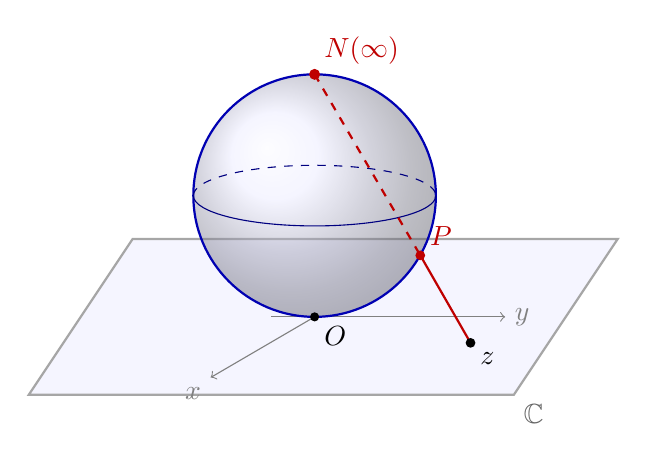
\begin{tikzpicture}[scale=1.1]
    % Complex plane
    \draw[thick, gray!70, fill=blue!4] (-3.2,-1.2) -- (2.4,-1.2) -- (3.6,0.6) -- (-2.0,0.6) -- cycle;
    \node[below right, gray!80!black] at (2.4,-1.2) {$\mathbb{C}$};

    % Coordinate axes on plane
    \draw[->, thin, gray] (-0.4,-0.3) -- (2.3,-0.3) node[right] {$y$};
    \draw[->, thin, gray] (0.1,-0.3) -- (-1.1,-1.0) node[below left] {$x$};

    % Sphere centered at (0.1, 1.1) with radius 1.4
    \def\cx{0.1}
    \def\cy{1.1}
    \def\rad{1.4}
    \shade[ball color=blue!12, opacity=0.45] (\cx,\cy) circle (\rad);
    \draw[thick, blue!70!black] (\cx,\cy) circle (\rad);
    \draw[dashed, blue!50!black] (\cx-\rad,\cy) arc (180:0:\rad cm and 0.35cm);
    \draw[blue!50!black] (\cx-\rad,\cy) arc (180:360:\rad cm and 0.35cm);

    % Poles O and N
    \fill[black] (\cx, \cy-\rad) circle (1.5pt) node[below right] {$O$};
    \fill[red!75!black] (\cx, \cy+\rad) circle (1.8pt) node[above right] {$N(\infty)$};

    % Projection line N - P - Z
    \coordinate (N) at (\cx, \cy+\rad);
    \coordinate (Z) at (1.9, -0.6);
    \coordinate (P) at (1.32, 0.41);

    \draw[dashed, red!75!black, thick] (N) -- (P);
    \draw[red!75!black, thick] (P) -- (Z);

    \fill[black] (Z) circle (1.6pt) node[below right] {$z$};
    \fill[red!75!black] (P) circle (1.6pt) node[above right] {$P$};
\end{tikzpicture}
\caption{Stereographic projection establishing a bijection between $\mathbb{C}_\infty$ and the Riemann sphere.}
\end{figure}

\textbf{Geometric Properties on the Riemann Sphere}:
\begin{itemize}
    \item Every straight line in $\mathbb{C}$ corresponds to a circle on the Riemann sphere passing through the North Pole $N$; hence, every straight line in $\mathbb{C}_\infty$ passes through $\infty$.
    \item No open half-plane in $\mathbb{C}$ contains the point $\infty$.
\end{itemize}

\subsection{Topological Concepts in $\mathbb{C}_\infty$}

\begin{definition}[Neighborhood of $\infty$]
In the extended complex plane $\mathbb{C}_\infty$, the $\varepsilon$-neighborhood of $\infty$ is defined as the exterior of a disk centered at the origin:
\[
    N(\infty, \varepsilon) = \left\{ z \in \mathbb{C}_\infty \,\middle|\, |z| > \frac{1}{\varepsilon} \right\} \quad (\text{or } \{ |z| > R \} \text{ for } R > 0).
\]
The deleted neighborhood of $\infty$ is $\mathring{N}(\infty, \varepsilon) = \left\{ z \in \mathbb{C} \,\middle|\, |z| > \frac{1}{\varepsilon} \right\}$.
\end{definition}

\textbf{Key Topological Remarks for $\mathbb{C}_\infty$}:
\begin{itemize}
    \item \textbf{Boundary Orientation of $\{|z| > R\}$}: When considering the exterior domain $D = \{ |z| > R \}$ in $\mathbb{C}_\infty$, keeping $D$ on the left requires traversing the circle $|z| = R$ in the \textbf{clockwise} direction, denoted by $\Gamma^- = \{ |z| = R \}^-$.
    \item \textbf{Boundary of $\mathbb{C}$}: In $\mathbb{C}_\infty$, the finite complex plane $\mathbb{C}$ has $\infty$ as its sole boundary point, whereas $\mathbb{C}_\infty$ itself is a domain without boundary (with $\infty$ as an interior point).
    \item \textbf{Simply Connectedness in $\mathbb{C}_\infty$}: A simple closed curve $C$ inside a domain $D \subset \mathbb{C}_\infty$ can continuously shrink to $\infty$ by expanding into arbitrarily small neighborhoods $\{|z| > R\}$ of $\infty$. Consequently, $\{|z| > 1\}$ is \textbf{simply connected} in $\mathbb{C}_\infty$, whereas the punctured exterior $\{1 < |z| < +\infty\}$ is \textbf{multiply connected}.
\end{itemize}

% ==================================================
% Section 3: Functions of a Complex Variable
% ==================================================
\section{Functions of a Complex Variable}

\subsection{Concept of Complex Functions and Geometric Mappings}

\begin{definition}[Complex Function]
Let $D$ be a point set in the complex plane $\mathbb{C}$. If for every complex number $z \in D$, there corresponds one or more complex numbers $w$ according to a rule $f$, then $w$ is called a \textbf{function of a complex variable} defined on $D$, denoted by
\[
    w = f(z), \quad z \in D.
\]
Here $D$ is the \textbf{domain of definition}, and $G = \{ w = f(z) \mid z \in D \}$ is the \textbf{range} (image set).
\end{definition}

\textbf{Structural and Geometric Properties}:
\begin{itemize}
    \item \textbf{Single-valued vs. Multi-valued Functions}: If each $z \in D$ corresponds to a unique value $w$, $f(z)$ is called \emph{single-valued} (e.g., $w = z^2$, $w = |z|$); if $z$ corresponds to two or more values, $f(z)$ is called \emph{multi-valued} (e.g., $w = \operatorname{Arg} z$, $w = \sqrt[n]{z}$).
    \item \textbf{Real and Imaginary Decomposition}: Writing $z = x + iy$ and $w = u + iv$, a complex function is equivalent to a pair of real-valued functions of two real variables:
    \[
        w = f(z) = u(x, y) + i v(x, y).
    \]
    \item \textbf{Inverse Function}: If for each $w \in G$ there exist one or more points $z \in D$ satisfying $w = f(z)$, this correspondence defines the inverse function $z = g(w) = f^{-1}(w)$.
    \item \textbf{Geometric Interpretation as a Mapping}: Unlike a real function $y = f(x)$ which can be visualized as a curve in $\mathbb{R}^2$, a complex function $w = f(z)$ involves four real variables $(x, y, u, v)$ and cannot be plotted as a graph in low dimensions. Instead, we interpret $w = f(z)$ as a \textbf{mapping} (or transformation) from a set $D$ in the $z$-plane to its image $G$ in the $w$-plane (which may be injective/one-to-one, surjective/onto, or bijective).
\end{itemize}

\begin{example}[Mapping Properties of $w = z^2$]
Let $z = x + iy = r e^{i\theta}$ and $w = u + iv = \rho e^{i\varphi}$. For $w = z^2$, we have
\[
    u = x^2 - y^2, \quad v = 2xy \qquad \text{and} \qquad \rho = r^2, \quad \varphi = 2\theta + 2k\pi.
\]
\begin{enumerate}
    \item \textbf{Image of the Real Axis}: On the real axis $y = 0$, we obtain $u = x^2 \ge 0$ and $v = 0$. Thus, $w = z^2$ maps the real axis of the $z$-plane onto the non-negative real axis $[0, +\infty)$ of the $w$-plane (covering $(0, +\infty)$ twice, once for $x > 0$ and once for $x < 0$). Similarly, the imaginary axis $x = 0$ maps onto the non-positive real axis $(-\infty, 0]$.
    \item \textbf{Image of Angular Sectors}: The angular sector $0 < \arg z < \alpha$ ($0 < \alpha \le \pi$) is mapped onto the sector $0 < \arg w < 2\alpha$. In particular, the first quadrant $0 < \arg z < \frac{\pi}{2}$ is mapped one-to-one onto the upper half-plane $0 < \arg w < \pi$.
\end{enumerate}
\end{example}

\subsection{Elementary Complex Functions}

Elementary functions of a complex variable are grouped into \textbf{five major categories}, extending real elementary functions to $\mathbb{C}$ while preserving algebraic identities.

\subsubsection{1. Exponential Function}

\begin{definition}[Complex Exponential Function]
For any complex number $z = x + iy$, the exponential function is defined by
\[
    w = e^z = \exp(z) = e^{x + iy} = e^x (\cos y + i \sin y).
\]
\end{definition}

\textbf{Properties of $e^z$}:
\begin{enumerate}
    \item \textbf{Modulus and Argument}: $|e^z| = e^x > 0$ (hence $e^z \neq 0$ for all $z \in \mathbb{C}$), and $\operatorname{Arg}(e^z) = y + 2k\pi$ ($k \in \mathbb{Z}$).
    \item \textbf{Real, Imaginary, and Conjugate Parts}:
    \[
        \operatorname{Re}(e^z) = e^x \cos y, \quad \operatorname{Im}(e^z) = e^x \sin y, \quad \overline{e^z} = e^x(\cos y - i\sin y) = e^{\overline{z}}.
    \]
    \item \textbf{Addition Property}: For all $z_1, z_2 \in \mathbb{C}$, $e^{z_1} \cdot e^{z_2} = e^{z_1 + z_2}$. (Note: $(e^{z_1})^{z_2} = e^{z_1 z_2}$ does not hold in general due to multi-valuedness.)
    \item \textbf{Periodicity}: Since $e^{2k\pi i} = 1$, $e^z$ is periodic with fundamental period $T = 2\pi i$:
    \[
        e^{z + 2k\pi i} = e^z \quad (k = 0, \pm 1, \pm 2, \dots).
    \]
    \item \textbf{Analyticity and Behavior at $\infty$}: $e^z$ is analytic on the entire complex plane $\mathbb{C}$ with $(e^z)' = e^z$, and $\lim_{z \to \infty} e^z$ does not exist.
\end{enumerate}

\subsubsection{2. Logarithmic Function}

\begin{definition}[Complex Logarithmic Function]
For $z \neq 0, \infty$, any complex number $w$ satisfying $e^w = z$ is called the logarithm of $z$, denoted by $w = \operatorname{Ln} z$. Writing $z = r e^{i\theta}$ and $w = u + iv$, we obtain
\[
    w = \operatorname{Ln} z = \ln|z| + i\operatorname{Arg} z = \ln|z| + i(\arg z + 2k\pi) \quad (k = 0, \pm 1, \pm 2, \dots).
\]
\end{definition}

\textbf{Properties of $\operatorname{Ln} z$}:
\begin{enumerate}
    \item \textbf{Principal Value and Branches}: Fixing $k$ yields a single-valued branch. For $k = 0$, we obtain the \textbf{principal value}:
    \[
        \ln z = \ln|z| + i\arg z \quad (-\pi < \arg z \le \pi),
    \]
    where $\operatorname{Re}(\ln z) = \ln|z|$ and $\operatorname{Im}(\ln z) = \arg z$. Thus $\operatorname{Ln} z = \ln z + 2k\pi i$.
    \item \textbf{Example}: $\operatorname{Ln}(-1) = \ln|-1| + i(\pi + 2k\pi) = (2k + 1)\pi i$, with principal value $\ln(-1) = \pi i$.
    \item \textbf{Algebraic Identities}: For $z_1, z_2 \neq 0$, as equalities between sets of values:
    \[
        \operatorname{Ln}(z_1 z_2) = \operatorname{Ln} z_1 + \operatorname{Ln} z_2, \qquad \operatorname{Ln}\left(\frac{z_1}{z_2}\right) = \operatorname{Ln} z_1 - \operatorname{Ln} z_2.
    \]
    \emph{Warning}: For principal values, $\ln(z_1 z_2) = \ln z_1 + \ln z_2$ \textbf{does not always hold} (e.g., when $\arg z_1 + \arg z_2 \notin (-\pi, \pi]$).
    \item \textbf{Analyticity}: Every branch of $\operatorname{Ln} z$ is analytic on the slit plane $\mathbb{C} \setminus (-\infty, 0]$ with derivative $(\operatorname{Ln} z)' = \frac{1}{z}$.
\end{enumerate}

\subsubsection{3. Power Function and General Exponential Function}

\begin{definition}[Complex Power Function]
For any complex exponent $a \in \mathbb{C}$ and $z \neq 0$, the power function is defined via the exponential and logarithmic functions as
\[
    w = z^a = e^{a \operatorname{Ln} z} = e^{a(\ln|z| + i\arg z + 2k\pi i)} = e^{a \ln z} \cdot e^{2k\pi a i} \quad (k = 0, \pm 1, \pm 2, \dots).
\]
Similarly, for $a \neq 0$, the general exponential function is defined as $w = a^z = e^{z \operatorname{Ln} a}$ (which is multi-valued when $a \neq e$).
\end{definition}

\textbf{Classification by Exponent $a$}:
\begin{itemize}
    \item $a = n \in \mathbb{Z}^+$: $w = z^n = r^n e^{in\theta}$ is single-valued and entire on $\mathbb{C}$.
    \item $a = -n$ ($n \in \mathbb{Z}^+$): $w = z^{-n} = \frac{1}{z^n}$ is single-valued and analytic on $\mathbb{C} \setminus \{0\}$.
    \item $a = \frac{1}{n}$ ($n \in \mathbb{Z}^+$): $w = z^{1/n} = \sqrt[n]{z} = \sqrt[n]{r} e^{i\frac{\theta + 2k\pi}{n}}$ ($k = 0, 1, \dots, n-1$) is $n$-valued.
    \item $a = \frac{m}{n}$ (reduced fraction, $n > 1$): $w = z^{m/n}$ is $n$-valued.
    \item Other $a$ (irrational or non-real complex): $w = z^a$ is infinitely many-valued.
\end{itemize}

\begin{example}[Evaluation of $i^i$]
Compute all values of the multi-valued power $i^i$:
\[
    i^i = e^{i \operatorname{Ln} i} = e^{i\left[\ln|i| + i\left(\frac{\pi}{2} + 2k\pi\right)\right]} = e^{-\frac{\pi}{2} - 2k\pi} \quad (k = 0, \pm 1, \pm 2, \dots).
\]
Notice that all infinitely many values of $i^i$ are positive real numbers!
\end{example}

\subsubsection{4. Trigonometric and Hyperbolic Functions}

\begin{definition}[Complex Trigonometric Functions]
Extending Euler's formula $e^{ix} = \cos x + i\sin x$ ($x \in \mathbb{R}$) to $z \in \mathbb{C}$, the sine and cosine functions are defined as
\[
    \sin z = \frac{e^{iz} - e^{-iz}}{2i}, \qquad \cos z = \frac{e^{iz} + e^{-iz}}{2}.
\]
The remaining trigonometric functions are defined by
\[
    \tan z = \frac{\sin z}{\cos z}, \quad \cot z = \frac{\cos z}{\sin z}, \quad \sec z = \frac{1}{\cos z}, \quad \csc z = \frac{1}{\sin z}.
\]
\end{definition}

\textbf{Properties of Complex Trigonometric Functions}:
\begin{enumerate}
    \item \textbf{Euler's Formula}: $e^{iz} = \cos z + i\sin z$ holds for all $z \in \mathbb{C}$.
    \item \textbf{Periodicity and Parity}: $\sin z$ and $\cos z$ are periodic with period $2\pi$; $\sin(-z) = -\sin z$ (odd) and $\cos(-z) = \cos z$ (even).
    \item \textbf{Analyticity and Identities}: $\sin z$ and $\cos z$ are entire functions with $(\sin z)' = \cos z$ and $(\cos z)' = -\sin z$. Standard real identities ($\sin^2 z + \cos^2 z = 1$, sum/difference formulas) remain valid.
    \item \textbf{Zeros}: All zeros lie on the real axis: $\sin z = 0 \iff z = k\pi$, and $\cos z = 0 \iff z = k\pi + \frac{\pi}{2}$ ($k \in \mathbb{Z}$).
    \item \textbf{Unboundedness}: Unlike real sine and cosine, $|\sin z|$ and $|\cos z|$ are \textbf{unbounded} on $\mathbb{C}$ (e.g., $|\cos(iy)| = \cosh y \to +\infty$ as $|y| \to \infty$).
\end{enumerate}

\begin{definition}[Complex Hyperbolic Functions]
The hyperbolic sine, cosine, and tangent functions are defined for $z \in \mathbb{C}$ by
\[
    \sinh z = \frac{e^z - e^{-z}}{2}, \qquad \cosh z = \frac{e^z + e^{-z}}{2}, \qquad \tanh z = \frac{\sinh z}{\cosh z}.
\]
\end{definition}

They satisfy $\sinh z = -i\sin(iz)$, $\cosh z = \cos(iz)$, $\cosh^2 z - \sinh^2 z = 1$, $(\sinh z)' = \cosh z$, and $(\cosh z)' = \sinh z$, with fundamental period $2\pi i$.

\subsubsection{5. Inverse Trigonometric and Inverse Hyperbolic Functions}

Defined as the inverse mappings of the trigonometric and hyperbolic functions, these functions are all infinitely many-valued:
\begin{align*}
    \operatorname{Arcsin} z &= -i\operatorname{Ln}\left(iz \pm \sqrt{1 - z^2}\right), & \operatorname{Arccos} z &= -i\operatorname{Ln}\left(z \pm \sqrt{z^2 - 1}\right), \\[6pt]
    \operatorname{Arctan} z &= -\frac{i}{2}\operatorname{Ln}\frac{1 + iz}{1 - iz} \quad (z \neq \pm i), & \operatorname{Arccot} z &= \frac{i}{2}\operatorname{Ln}\frac{z - i}{z + i} \quad (z \neq \pm i), \\[6pt]
    \operatorname{Arcsinh} z &= \operatorname{Ln}\left(z \pm \sqrt{z^2 + 1}\right), & \operatorname{Arccosh} z &= \operatorname{Ln}\left(z \pm \sqrt{z^2 - 1}\right).
\end{align*}

% ==================================================
% Section 4: Assigned Exercises Reference
% ==================================================
\vspace{0.8em}
\noindent\rule{\textwidth}{0.5pt}
\section*{Assigned Homework Reference}
\begin{itemize}
    \item \textbf{Textbook P.20 (Exercise 1)}: Set A: Problems 8 (even), 9, 12; \quad Set B: Problems 5, 6.
    \item \textbf{Textbook P.55 (Exercise 2)}: Set A: Problem 13 (even).
\end{itemize}

\end{document}